\documentclass[a4j,twoside,openright,11pt]{jarticle}
%
\usepackage{amsmath,amssymb}
\usepackage{bm}
\usepackage{graphicx}
\usepackage{ascmac}
\usepackage{listliketab}
\usepackage{url}
\usepackage{listings}

\setlength{\textwidth}{15.92cm}
\setlength{\oddsidemargin}{0mm}
\setlength{\evensidemargin}{0mm}
\setlength{\topmargin}{-1cm}
\setlength{\textheight}{23.5cm}
\setlength{\footskip}{18mm}

%
\pagestyle{plain}
\title{機械工学実験2\\3次元翼空力実験}
\author{九州工業大学 機械知能工学科 機械知能コース 3年\\学籍番号:13104069 坂本悠作 \\実験日1 2015年6月3日 \\ 実験日2 2015年6月10日}


\begin{document}
\maketitle
\newpage

\section{目的}
流体機械の主要素である3次元翼について、低速風洞試験設備を利用した力及び圧力の計測を行い、基本的な圧力特性や性能計算を理解する。

\section{実験装置と実験方法}
\subsection{実験装置}
\subsubsection{風洞}

\begin{table}[htb]
\begin{center}
  \caption{実験に用いた低速風洞試験設備の諸元}
  \begin{tabular}{ll} \hline
風洞型式                &閉鎖型回流式\\
測定部寸法              &$0.45m(幅)\times 0.45m(高さ) \times 1.35m(長さ) $\\
縮流比                  &1:4\\
風速範囲(閉鎖型回流式)  &$5 \sim 45 m/s$\\
風速範囲(開放型回流式)  &$5 \sim 40 m/s$\\
気流の流れ              &吹き出し口断面中心にて1.0\%以下\\
\hline
  \end{tabular}
\end{center}
\end{table}

\subsubsection{天秤}

\begin{table}[htb]
\begin{center}
  \caption{天秤の仕様}
  \begin{tabular}{ll} \hline
定格負荷                &$F_x \pm 100[N]$\\
                        &$F_y \pm 100[N]$\\
                        &$F_z \pm 100[N]$\\
非線形性                &$\pm 0.5 \% FS$\\
許容過負荷              &$\pm 150 \% FS$\\
零点の温度影響          &$\pm 0.01 \% FS/℃ $\\
感度の温度影響          &$\pm 0.01 \% Reading/℃$\\
日章電気(株)社製3分力計 &LMC-3501-100N\\
\hline
  \end{tabular}
\end{center}
\end{table}

\newpage
\subsubsection{32チャンネル圧力センサーユニット}
\begin{table}[htbp]
\begin{center}
  \caption{チャンネル圧力センサーユニットの仕様}
  \begin{tabular}{ll} \hline
定格出力                &$0 \sim +10Vdc at 0 \sim +7.5 kPa$\\
                        &$0 \sim -10Vdc at 0 \sim -7.5 kPa$\\
測定精度                &$\pm0.4\%F.S.$\\
温度影響(ゼロドリフト)  &$\pm 4mV/℃ at \,0 \sim 50 ℃ $\\
\,\,\,\,\,\,\,\,\,\,\,\,\,\,\,\,\,\,\,\,\,\,\,\,(スパンドリフト)&$\pm 5mV/℃ at \,0 \sim 50 ℃ $\\
OFFSET範囲              &$\pm 4mV/℃  atF.S. $\\
東亜工業株式会社製      &32チャンネル圧力センサーユニット\\
\hline
  \end{tabular}
\end{center}
\end{table}

\subsubsection{供試体}

\begin{table}[htb]
\begin{center}
  \caption{3次元翼の諸元}
  \begin{tabular}{ll} \hline
形態&片持ち半裁翼\\
平面形&矩形翼\\
翼型&NACA0012(対象翼)\\
半スパン長&210mm\\
翼弦長&70mm\\
主翼面積&$2.94 \times 10^{4}mm^2$\\
アスペクト比&6\\
圧力孔&反スパン中央位置の翼断面において\\
&上面10点、下面10点\\
\hline
  \end{tabular}
\end{center}
\end{table}
圧力孔の位置は、上面の2,6,12,20,30,40,50,60,75,90[\%翼弦長],下面の1,4,9,17,25,35,45,55,70,85[\%翼弦長]に配置してある。また、この翼型の翼弦長と翼厚の関係として、次の理論式が与えられている。
\begin{eqnarray}
\pm y = \frac{0.12}{0.20}\left(0.29690\sqrt{x} -0.12600x -0.35160x^2 +0.28430x^3 -0.10150x^4 \right)
\end{eqnarray}

\subsection{実験方法}
\subsubsection{力計測の手順}

\begin{enumerate}
\item アンプの電源を入れ、出力が安定するまで待つ(最低30分)
\item アンプの0設定及び測定レンジ合わせ
\item アンプの校正を行なう
\item ピトー管を設置する
\item 操作盤の周波数ダイアルを徐々に回して通風し、目標レイノルズ数となる送風機回転を調べる
\item 天秤に供試体を取り付け、風洞に設置する。
\item 水準器を用いて仰角$\alpha = 0$に設置する
\end{enumerate}


\subsubsection{圧力計速の手順}

\section{実験結果}
\subsection{力計測から得られたデータの整理}
\newpage
\begin{figure}[htbp]
\begin{center}
\includegraphics[width=9cm,angle=-90]{./CL/CL.eps}
\end{center}
\caption{$\alpha - C_L$}
\end{figure}

\begin{figure}[htbp]
\begin{center}
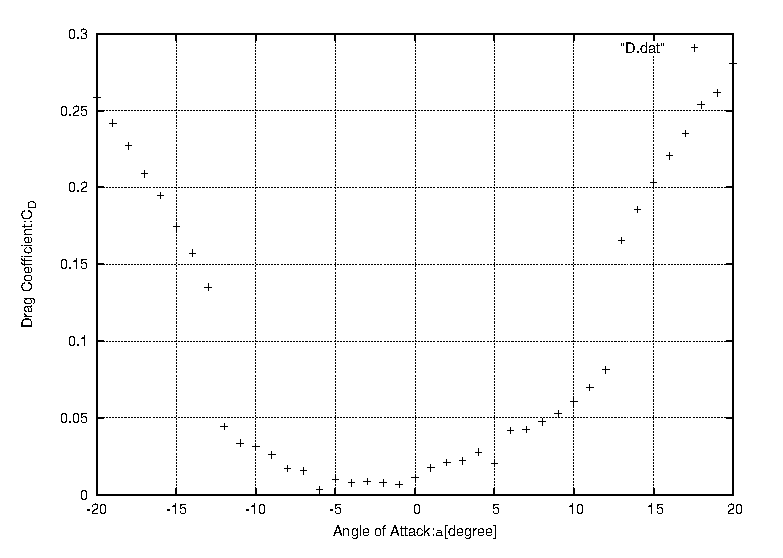
\includegraphics[width=9cm,angle=-90]{./CD/CD.eps}
\end{center}
\caption{$\alpha - C_D$}
\end{figure}

\begin{figure}[htbp]
\begin{center}
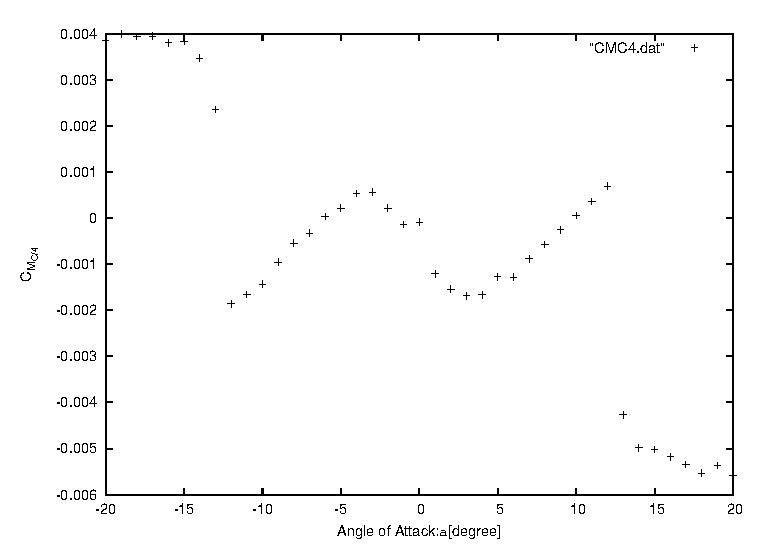
\includegraphics[width=12cm]{./CMC4/CMC4.eps}
\end{center}
\caption{$\alpha - C_{M_{C/4}}$}
\end{figure}

\begin{figure}[htbp]
\begin{center}
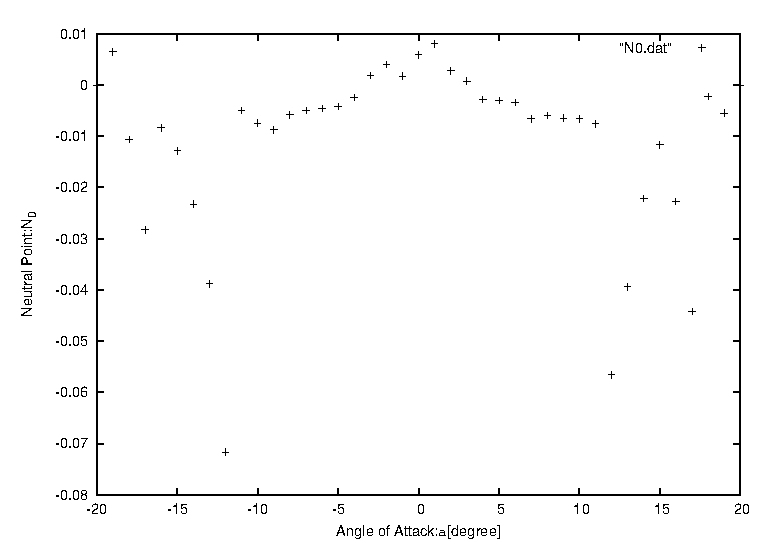
\includegraphics[width=12cm]{./N0/N0.eps}
\end{center}
\caption{$\alpha - N_0$}
\end{figure}

\begin{figure}[htbp]
\begin{center}
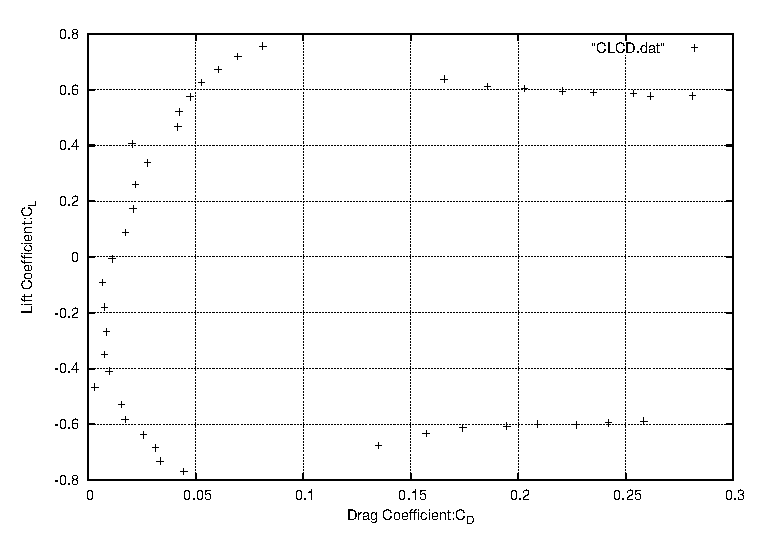
\includegraphics[width=12cm]{./CLCD/CLCD.eps}
\end{center}
\caption{$C_L - C_D$}
\end{figure}

\subsection{圧力計測から得られた圧力係数と圧力分布の整理}
得られた風洞制圧(大気圧)との差圧を、電圧からパスカルに変換する。このとき使用した32チャンネル圧力センサーユニットの仕様により、1[V]が750[Pa]であることを利用した。
\begin{figure}[htbp]
\begin{center}
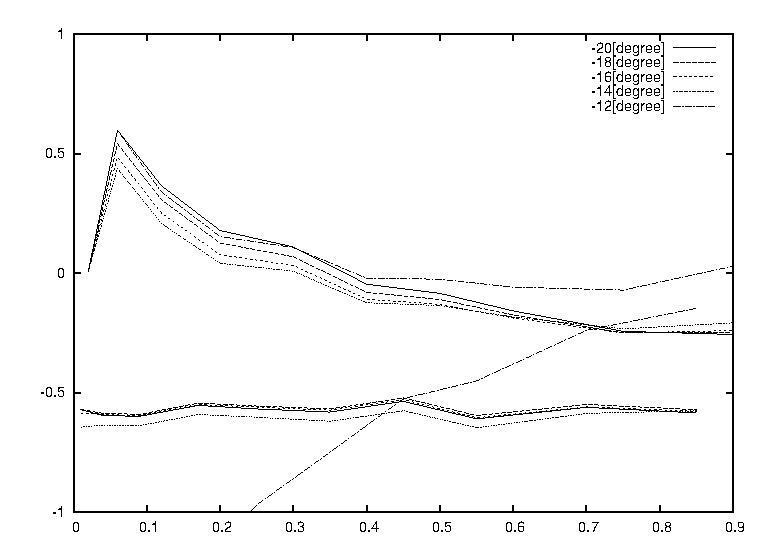
\includegraphics[width=12cm]{./2-CP/-20to-12.eps}
\end{center}
\caption{$-20to-12$}
\end{figure}

\begin{figure}[htbp]
\begin{center}
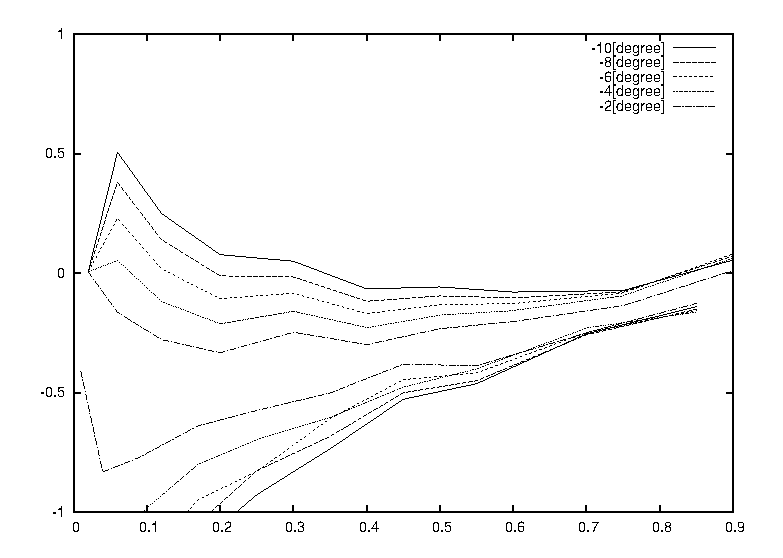
\includegraphics[width=12cm]{./2-CP/-10to-2.eps}
\end{center}
\caption{$-10to-2$}
\end{figure}

\begin{figure}[htbp]
\begin{center}
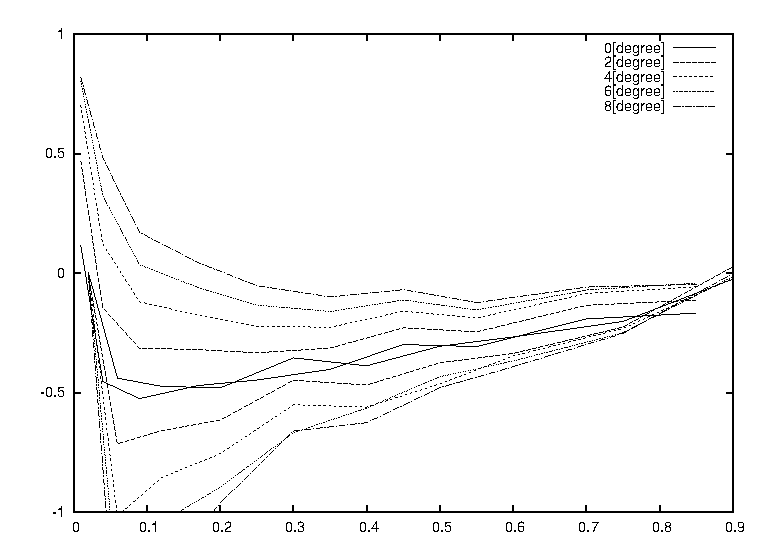
\includegraphics[width=12cm]{./2-CP/0to8.eps}
\end{center}
\caption{$0to8$}
\end{figure}

\begin{figure}[htbp]
\begin{center}
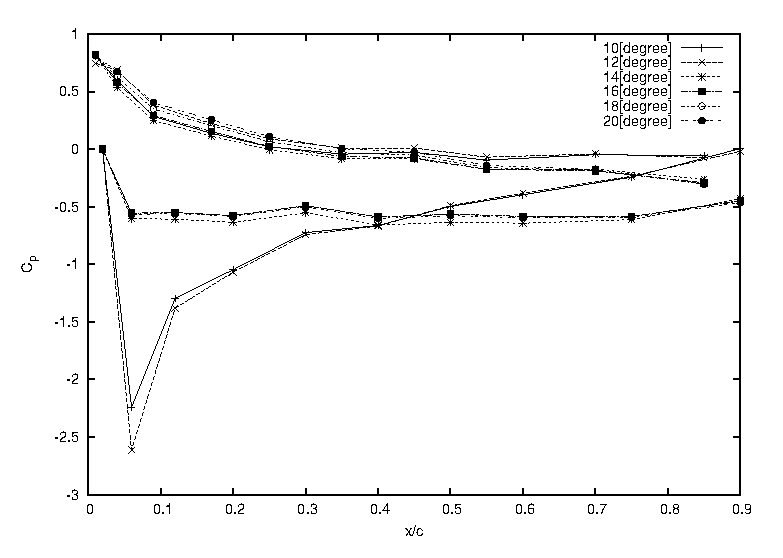
\includegraphics[width=12cm]{./2-CP/10-20.eps}
\end{center}
\caption{$10to20$}
\end{figure}

今回の実験で使用した翼型NACA0012の理論式を以下に示す。
\begin{eqnarray}
\pm y = \frac{0.12}{0.20}\left(0.29690\sqrt{x} -0.12600x -0.35160x^2 +0.28430x^3 -0.10150x^4 \right)
\end{eqnarray}
今、翼のy軸に対して翼表面の傾きについて求めたい。これを求めるのに以下の式を用いる。
\begin{eqnarray}
\tan \theta_i= \frac{dy}{dx}|_i
\end{eqnarray}
よって、$\theta$を算出するにはyの理論式を微分したものに$arctan$によって$\theta$を算出する。計算結果は以下の通りである。
\begin{eqnarray}
\frac{dy}{dx} = -0.126+\frac{0.14845}{\sqrt x}-0.7032x+0.8529x^2-0.406x^3
\end{eqnarray}

また、各面積にかかる力を算出するため、圧力孔付近に局所面積$\Delta s_i$を設ける。その値は求まった角度$\theta$を用いて次の式で算出した。

\begin{eqnarray}
\Delta s_i = c \times \frac{x_{i+1} - x_{i-1}}{2} \times \arccos \theta
\end{eqnarray}

\begin{table}[htb]
\begin{center}
  \caption{$\theta$の算出}
  \begin{tabular}{|l||c|c|c|c|} \hline
i&x&y'&θ[radian]&$\Delta s$\\\hline
1&0.02&0.5459843572&0.499754957&0.002199709\\
2&0.06&0.2645011987&0.2585796015&0.0045823569\\
3&0.12&0.1378406576&0.1369774836&0.0070235955\\
4&0.2&0.0577033748&0.0576394578&0.0095326869\\
5&0.3&-7.77726767161646E-005&-7.77726765593596E-005&0.0109961187\\
6&0.4&-0.0372479644&-0.0372307527&0.0112562498\\
7&0.5&-0.063110998&-0.0630274073&0.0114370588\\
8&0.6&-0.0821543245&-0.0819702404&0.0144625131\\
9&0.75&-0.104105823&-0.1037321496&0.0175845119\\
10&0.9&-0.1245149763&-0.1238774042&0.0148311867\\
11&0.01&0.8109317304&0.6813711777&0.0011496268\\
12&0.04&0.3536763936&0.3399462412&0.0034270225\\
13&0.09&0.1872947096&0.1851496244&0.0062998036\\
14&0.17&0.0822925604&0.0821075481&0.0083361389\\
15&0.25&0.0252375&0.0252321439&0.0097370375\\
16&0.35&-0.0204724211&-0.0204695616&0.0111388712\\
17&0.45&-0.0512569835&-0.0512121653&0.0113542163\\
18&0.55&-0.0732816365&-0.0731508786&0.0143851103\\
19&0.7&-0.0972871878&-0.0969819846&0.0175132754\\
20&0.85&-0.1174907206&-0.1169545379&0.017724201\\
\hline
  \end{tabular}
\end{center}
\end{table}

\begin{figure}[htbp]
\begin{center}
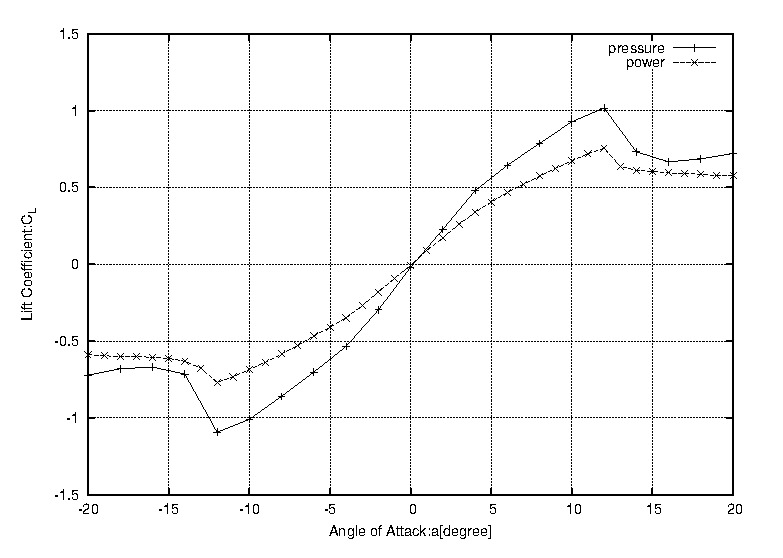
\includegraphics[width=12cm]{./2-CL-CD/CL-CD.eps}
\end{center}
\caption{$\alpha-C_L$}
\end{figure}

\begin{figure}[htbp]
\begin{center}
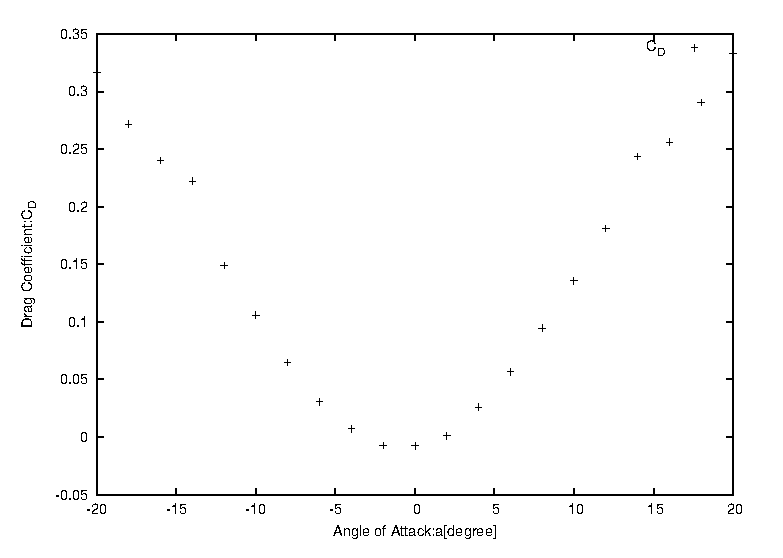
\includegraphics[width=12cm]{./2-CL-CD/CD.eps}
\end{center}
\caption{$\alpha-C_D$}
\end{figure}

\newpage
\section{考察}
\section{まとめ}
\section{参考文献}
機械工学実験2実験書
\section{風洞実験に対する感想・要望}
物体が受ける風の影響は、飛行機に限らず車やバイクなどの高速で移動する物質を制作する上で無視できないものであるので、機械実験で簡単に体験できたのは良い経験となりました。
\end{document}
